\chapter{Motivation \& Outline}\label{motivation}

Drug repositioning is time-efficient and less costly compared to traditional drug design processes. Computational methods are applied for drug repositioning to generate hypotheses for new indications for a drug candidate. With powerful algorithms and models, the process of drug design could be even shorter. As introduced in Biological Background, Himmelstein extract engineered feature vectors form Hetionet then train a logistic regression model to differentiate and predict whether drug-disease edge should exist in network.

Engineered features are more interpretable, but it takes lots of time to engineer and choose them, also lose much information like the neighbors and topological structure. If learned features with network representation learning are applied, it would be much easier for generating embeddings, tuning hyperparameters (e.g., dimensions) and keeping information. Muslu et al. ~\cite{muslu_guiltytargets:_2019} created protein-protein interaction network with differential gene expression as attribute to prioritize targets for diseases (Figure 7). They used learned features generated from DeepWalk to train a logistic regression model and got AUC-ROC values between 0.92 - 0.94.

\begin{figure}[!ht]
    \centering
    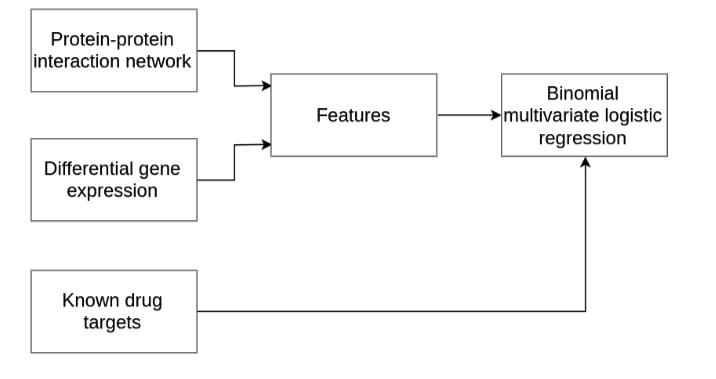
\includegraphics[scale=0.3]
    {figures/guiltytargets.png}
    \captionsetup{justification=centering}
    \caption[Workflow of GuiltyTargets]{\label{fig:guiltytargets} Workflow of GuiltyTargets. Figure adapted from ~\cite{muslu_guiltytargets:_2019}}
\end{figure}

These two work inspired the idea that replacing engineered features with learned features, then compare evaluation results between two embedding methods (Figure 8). At last, predict new drug-disease pairs with well tuned models trained by learned features.

\begin{figure}[!ht]
    \centering
    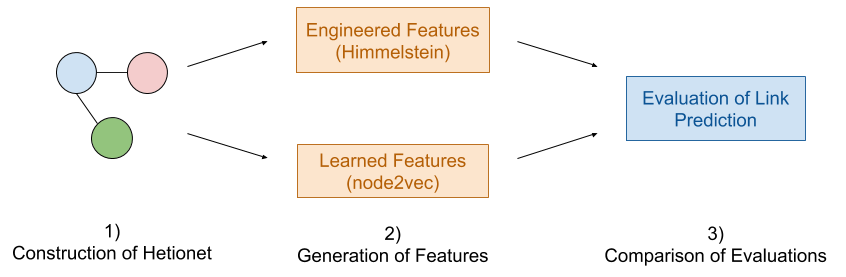
\includegraphics[scale=0.4]
    {figures/workflow.png}
    \captionsetup{justification=centering}
    \caption[Comparison workflow between engineered features and learned features]{\label{fig:workflow} Comparison workflow between engineered features and learned features ~\cite{lingling_xu_comaprison_workflow.png_2019}}
\end{figure}


